\chapter{Design Architecture}
\label{chp:design}
% Talk about previous designs and why I didn't/couldn't choose them (continuous tracking and sending to server).
As discussed in \nameref{it:1}, the non-continuous server design was chosen. The continuous server would be more complex to design and implement than the non-continuous version. This is because a constant connection between the plugin and server was required. If the network connection was interrupted or disconnected then data would not be sent to the server. This means that a fail-safe protocol would have to be implemented, such as writing the unsent data to file. This fail-safe protocol implementation would be required for the non-continuous server anyway.

The server-side of the continuous design would also need to be more sophisticated. The server would have to know when a new project is being started, which project data is being received, and when a project is completed. The non-continuous server only required a method to submit the tracked data file.

\section{Final Design}
\autoref{fig:architecture-diagram} shows the interaction between each of the modules. The plugin only needs to track file changes in the editor. This data is saved to an XML file, which the user can submit to the server using the front-end web application. This requires authentication using Aberystwyth credentials. Once the file has been submitted, the back-end server converts the XML data to JSON and stores it in the MongoDB database. The post-processor is continually monitoring the database for new student submissions to process and update the database with the result.

\autoref{fig:sequence-diagram-student-plugin} shows a typical students' interaction with the plugin. Initially, when a student opens a project, the tracked files are checked for external changes. This is done by comparing each files last known contents (which is stored as a base 64 encoded value) with its current file contents. The difference is added to the list of changes for each file. A DocumentListener is then added to the project for listening to file changes. Each file change is identified and then added to the list of changes for that file. After every new change that is added, the files last known contents is updated (for checking external changes). The recorded data is saved any time a file is saved. File change tracking stops when the project is closed (or if the plugin is disabled or uninstalled).

\autoref{fig:sequence-diagram-student-server} shows the students interaction with the server. Once the project is completed. The student may login to the web application using their Aberystwyth University credentials. This authorisation is achieved using the LDAP server provided by Aberystwyth University. This requires the back-end server to be running on the Aberystwyth University network. The LDAP server returns if authentication was successful or not. If successful, then the student will be redirected to their dashboard. A query is sent to the database to retrieve all of the students' submissions. These submissions are then displayed in a table in the dashboard. Students can post new project submissions by uploading the XML file with additional meta data for identification in a form. The form is submitted via POST. The XML file is decrypted and added to the students submissions in the database. The user will be notified of success or failure via a flash message.

\autoref{fig:sequence-diagram-post-processor} \textit{NOTE: Not sure how much detail to do on the post-processor here.} Upon posting a new submission, the post-processor is trigged. The new submission is processed and the result is inserted back into the database.

TODO: Talk about the front-end design too. Make a diagram for the front-end application design.

\subsection{Data structure}
\textit{TODO: Make class diagram for the data structure}

\subsection{Front-end web application}
\textit{TODO: Create web app diagrams}

\begin{figure}[H]
  \centering
  \fbox{
    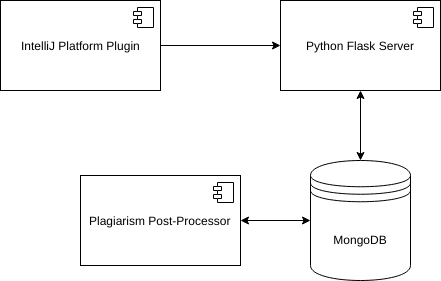
\includegraphics[height=.75\textheight,
    keepaspectratio=true,
    width=.75\textwidth,
    ]{figures/architecture-diagram.png}
  }
  \caption[Final design architecture diagram]{Architecture diagram (reminder to update this figure with descriptions for each component)}
  \label{fig:architecture-diagram}
\end{figure}

\begin{figure}[H]
  \centering
  \fbox{
    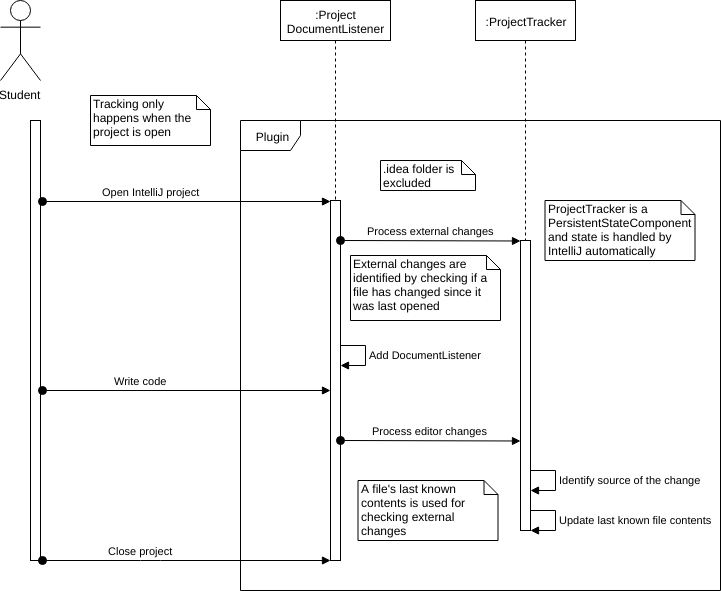
\includegraphics[height=.75\textheight,
    keepaspectratio=true,
    width=.75\textwidth,
    ]{figures/sequence-diagram-student-plugin.png}
  }
  \caption[Student-plugin sequence diagram]{Sequence diagram showing a student interacting with the IntelliJ plugin}
  \label{fig:sequence-diagram-student-plugin}
\end{figure}

\begin{figure}[H]
  \centering
  \fbox{
    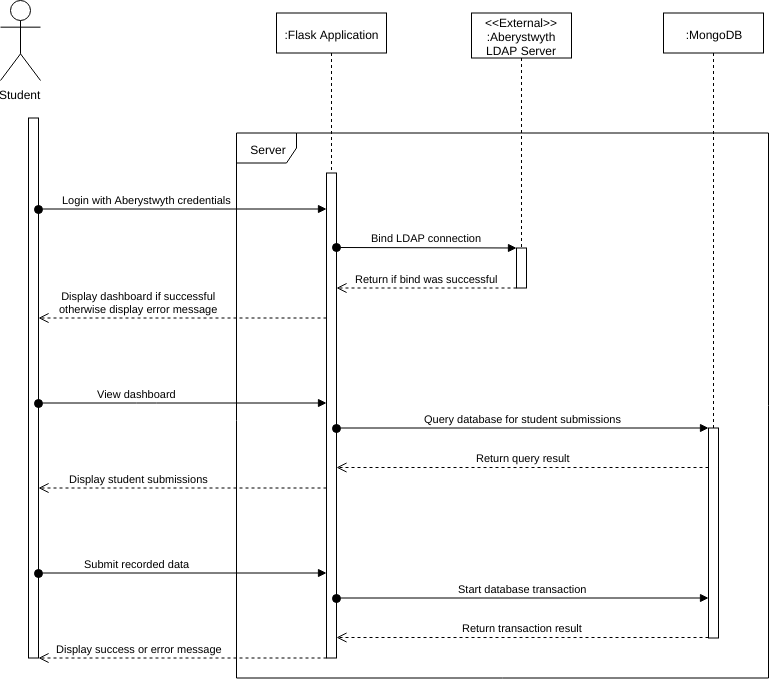
\includegraphics[height=.75\textheight,
    keepaspectratio=true,
    width=.75\textwidth,
    ]{figures/sequence-diagram-student-server.png}
  }
  \caption[Student-server sequence diagram]{Sequence diagram showing a student interacting with the server}
  \label{fig:sequence-diagram-student-server}
\end{figure}

\begin{figure}[H]
  \centering
  \fbox{
    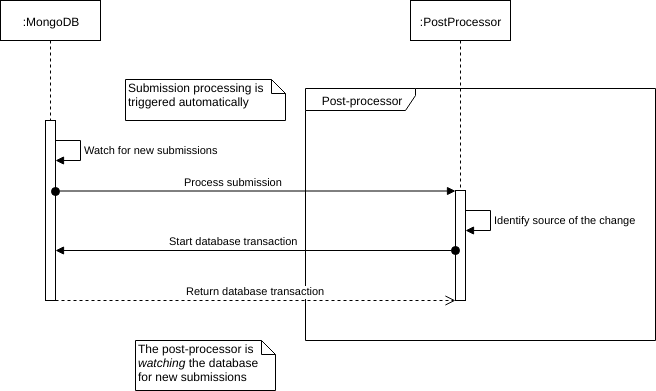
\includegraphics[height=.75\textheight,
    keepaspectratio=true,
    width=.75\textwidth,
    ]{figures/sequence-diagram-post-processor.png}
  }
  \caption[Post-processor sequence diagram]{Sequence diagram for the post-processor}
  \label{fig:sequence-diagram-post-processor}
\end{figure}
